\clearpage
\section*{ملحق: مطالبات المحكّم وأمثلة إضافية}
\label{app:judge-material}

\subsection*{تمييز التعليق المولد}
\begin{LTR}
{\footnotesize
\begin{verbatim}
Below is a discussion thread from r/{subreddit}, followed by 10 comments from that thread.
Exactly one comment was machine-generated and inserted. Identify it. Judge conversational
fit, specificity, stance, register, and habits; do not use length or polish as a cue.
Post title: {post_title}
Post body: {post_body}
Comments:
{numbered_comments}
Return JSON only:
{"inserted_index": INTEGER_1_TO_10,
 "confidence": INTEGER_0_TO_100,
 "runner_up_index": INTEGER_1_TO_10,
 "evidence": "SHORT_SENTENCE"}
\end{verbatim}
}
\end{LTR}

\subsection*{التعليق الأقل شبهًا بالبشري}
\begin{LTR}
{\footnotesize
\begin{verbatim}
Below is a discussion thread from r/{subreddit}, then three replies. Rank them from most
human-plausible (1) to least (3), then name the weakest. Ignore length and ordering.
Post title: {post_title}
Post body: {post_body}
Existing comments:
{numbered_context_comments}
Replies: 1‎. {candidate_1}
2‎. {candidate_2}
3‎. {candidate_3}
Return JSON only:
{"weakest_index": INTEGER_1_TO_3,
 "ranking": [INDEX, INDEX, INDEX],
 "evidence": "SHORT_SENTENCE"}
\end{verbatim}
}
\end{LTR}

\begin{figure}[H]
	\centering
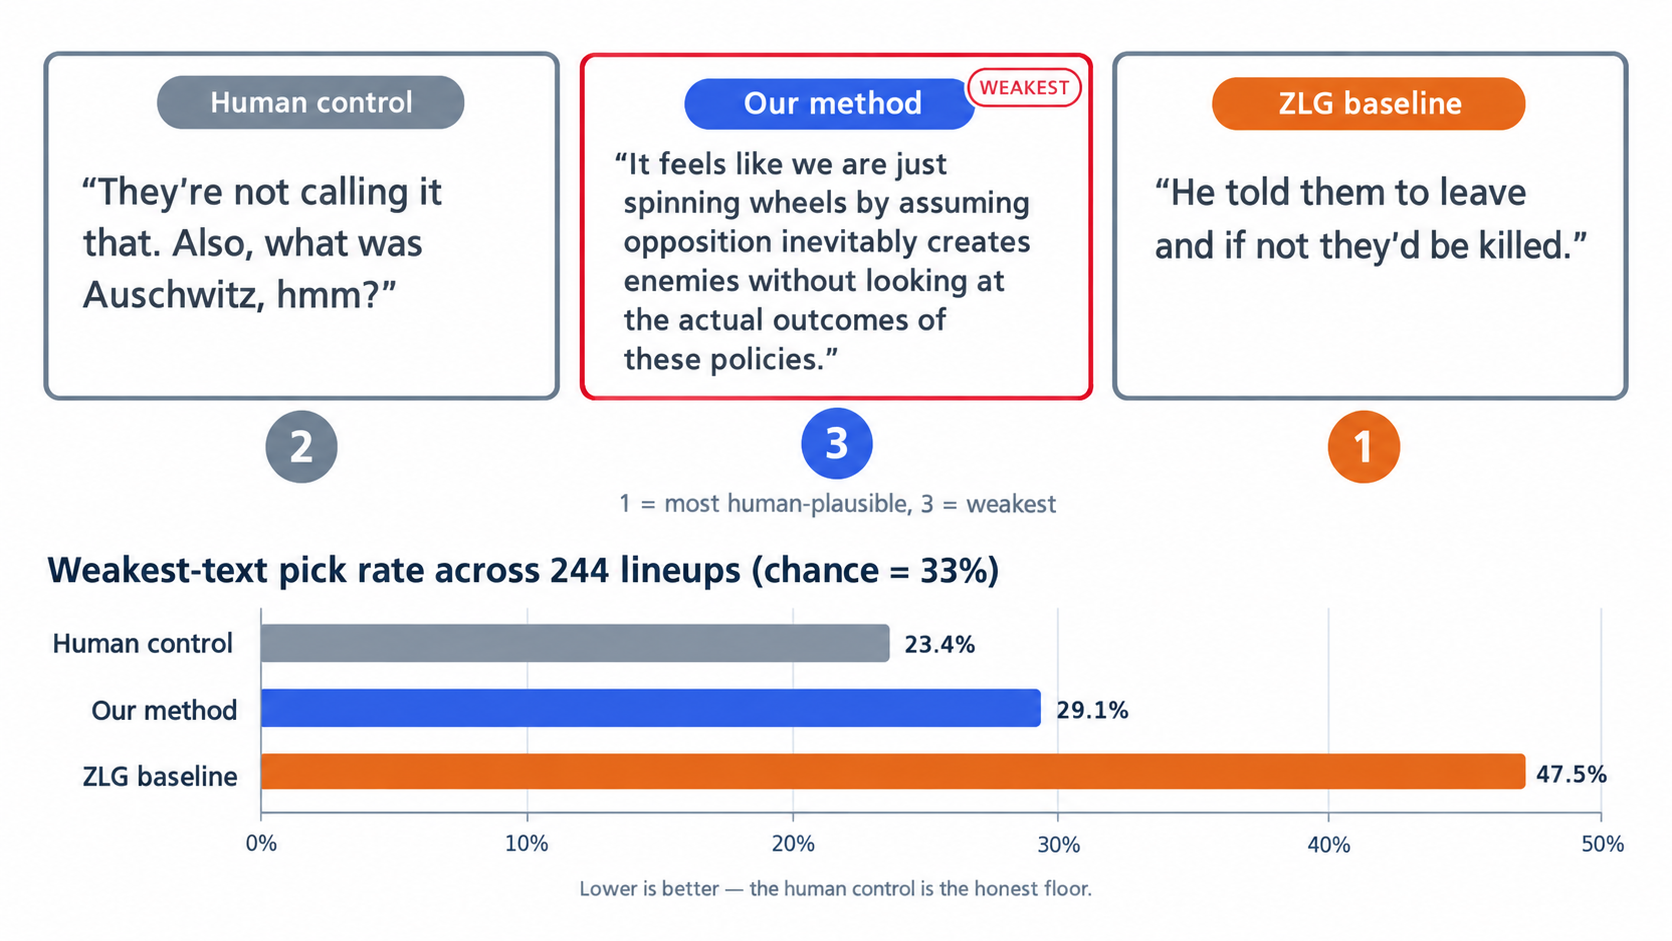
\includegraphics[width=\textwidth,height=0.55\textheight,keepaspectratio]{../common/figures/llm_judge_weakest_text}
	\caption{اختيار التعليق الأقل شبهًا بالبشري. اختار المحكّم تعليقنا في المثال المعروض، لكن عبر الأزواج الـ\NUM{244} اختار تعليق \EN{ZLG}~\cite{lin2024zero} أكثر (\NUM{47.5\%}) من تعليقنا (\NUM{29.1\%}) أو التعليق البشري (\NUM{23.4\%}).}
	\label{fig:judge-weak-link}
\end{figure}

\subsection*{درجة الاشتباه}
\begin{LTR}
{\footnotesize
\begin{verbatim}
You moderate r/{subreddit}. Score the reviewed comment from 0 (genuine human) to 100
(machine-generated or edited). Do not treat bluntness, mistakes, or poor punctuation
as evidence.
Post title: {post_title}
Post body: {post_body}
Recent comments:
{numbered_context_comments}
Comment: {candidate}
Select applicable tells from generic_could_fit_any_thread, ignores_thread_specifics,
register_mismatch, unnatural_phrasing, repetition, over_hedged, over_polished,
contradicts_thread_facts, none.
Return JSON only:
{"suspicion": INTEGER_0_TO_100,
 "tells": ["TELL"],
 "evidence": "SHORT_SENTENCE"}
\end{verbatim}
}
\end{LTR}

\begin{figure}[H]
	\centering
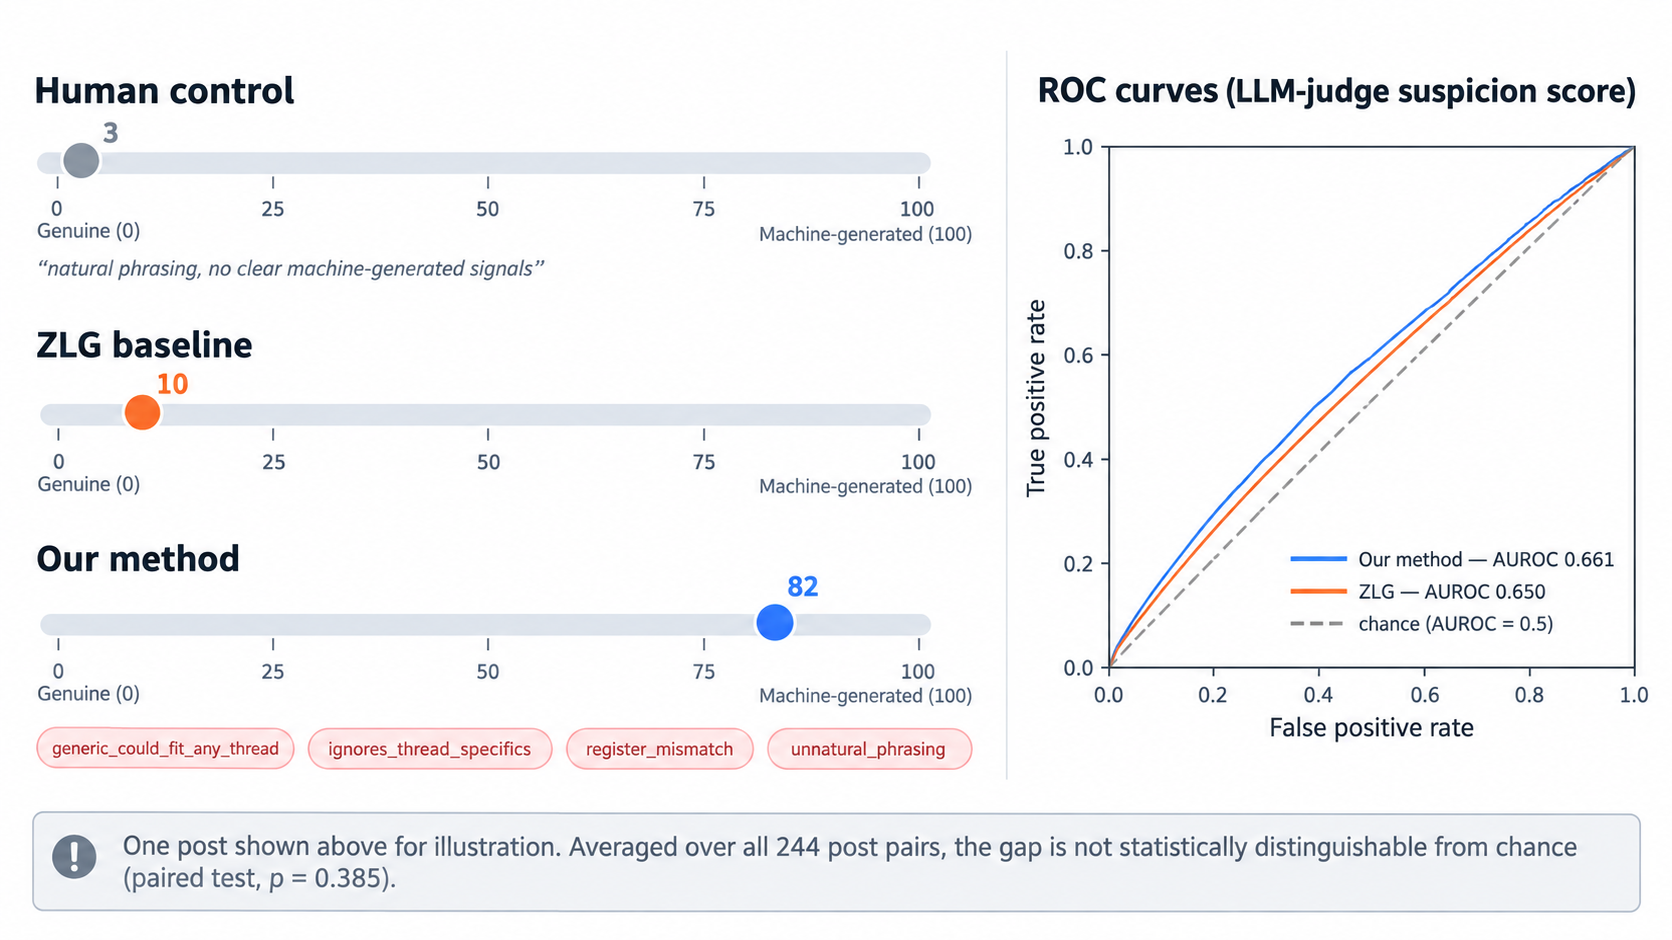
\includegraphics[width=\textwidth,height=0.55\textheight,keepaspectratio]{../common/figures/llm_judge_suspicion_auroc}
\caption{درجة الاشتباه، مثال من منشور واحد. أعطى المحكّم تعليقنا \NUM{82} وتعليق \EN{ZLG}~\cite{lin2024zero} عشر درجات. وعبر \NUM{244} زوجًا، بلغت قيمة \EN{AUROC} مقدار \NUM{0.661} لطريقتنا و\NUM{0.650} لـ\EN{ZLG}~\cite{lin2024zero}؛ أما اختبار درجات الاشتباه الخام المقترنة فلم يُظهر فرقًا واضحًا (\NUMM{p=0.385}).}
	\label{fig:judge-suspicion}
\end{figure}

\subsection*{إسناد التعليق إلى المحادثة}
\begin{LTR}
{\footnotesize
\begin{verbatim}
Below is a comment and four discussion threads. The comment belongs to exactly one thread.
Choose the most likely thread even if uncertain.
Comment: {candidate}
1‎. r/{sub_1} -- {title_1}
{snippet_1}
2‎. r/{sub_2} -- {title_2}
{snippet_2}
3‎. r/{sub_3} -- {title_3}
{snippet_3}
4‎. r/{sub_4} -- {title_4}
{snippet_4}
Return JSON only:
{"thread_index": INTEGER_1_TO_4,
 "confidence": INTEGER_0_TO_100,
 "evidence": "SHORT_SENTENCE"}
\end{verbatim}
}
\end{LTR}

\begin{figure}[H]
	\centering
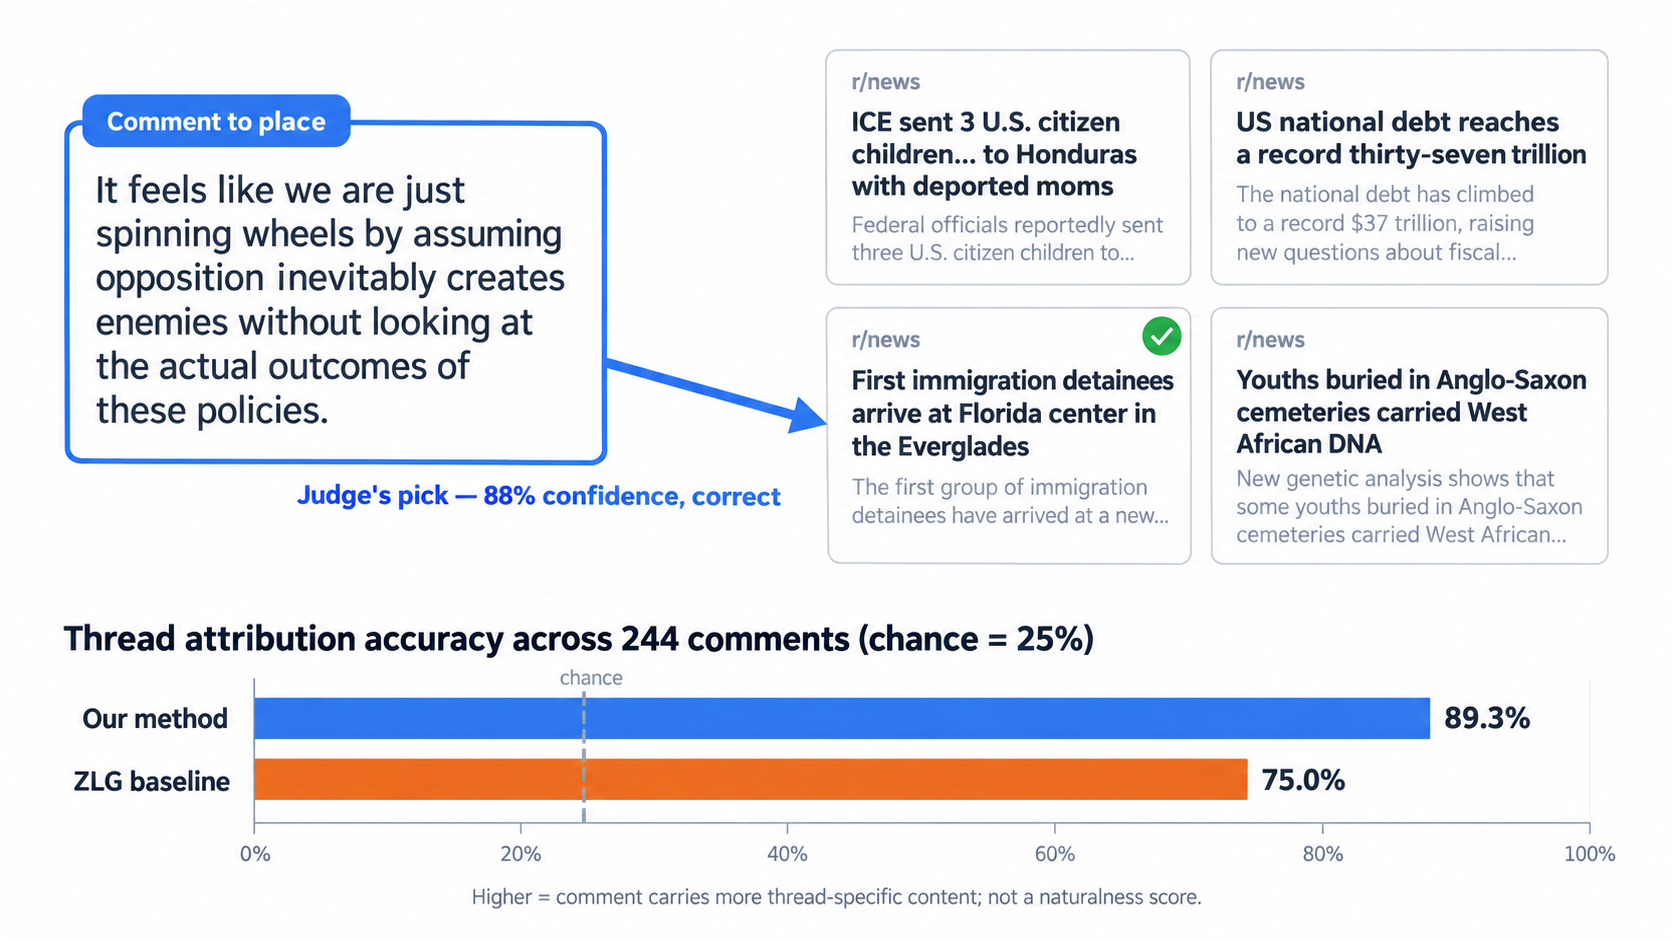
\includegraphics[width=\textwidth,height=0.55\textheight,keepaspectratio]{../common/figures/llm_judge_thread_attribution}
	\caption{إسناد التعليق إلى محادثته. في المثال المعروض، اختار المحكّم المحادثة الصحيحة لتعليقنا بثقة \NUM{88\%}. وعبر \NUM{244} تعليقًا لكل طريقة، بلغت الدقة \NUM{89.3\%} لطريقتنا و\NUM{75.0\%} لـ\EN{ZLG}~\cite{lin2024zero}؛ ويقيس ذلك ارتباط المحتوى بالمحادثة.}
	\label{fig:judge-attribution}
\end{figure}

\subsection*{ملاءمة السياق}
\begin{LTR}
{\footnotesize
\begin{verbatim}
Five genuine r/{subreddit} comments show the community register:
{numbered_context_comments}
Judge this comment's style only: {candidate}
Score tone_formality, length_norm, mechanics, insider_knowledge, and overall 1 (out of
place) to 5 (indistinguishable).
Schematic JSON shape only; numeric score placeholders:
{"tone_formality": INTEGER_1_TO_5, "length_norm": INTEGER_1_TO_5,
 "mechanics": INTEGER_1_TO_5, "insider_knowledge": INTEGER_1_TO_5,
 "overall": INTEGER_1_TO_5, "evidence": SHORT_SENTENCE}
\end{verbatim}
}
\end{LTR}

\begin{figure}[H]
	\centering
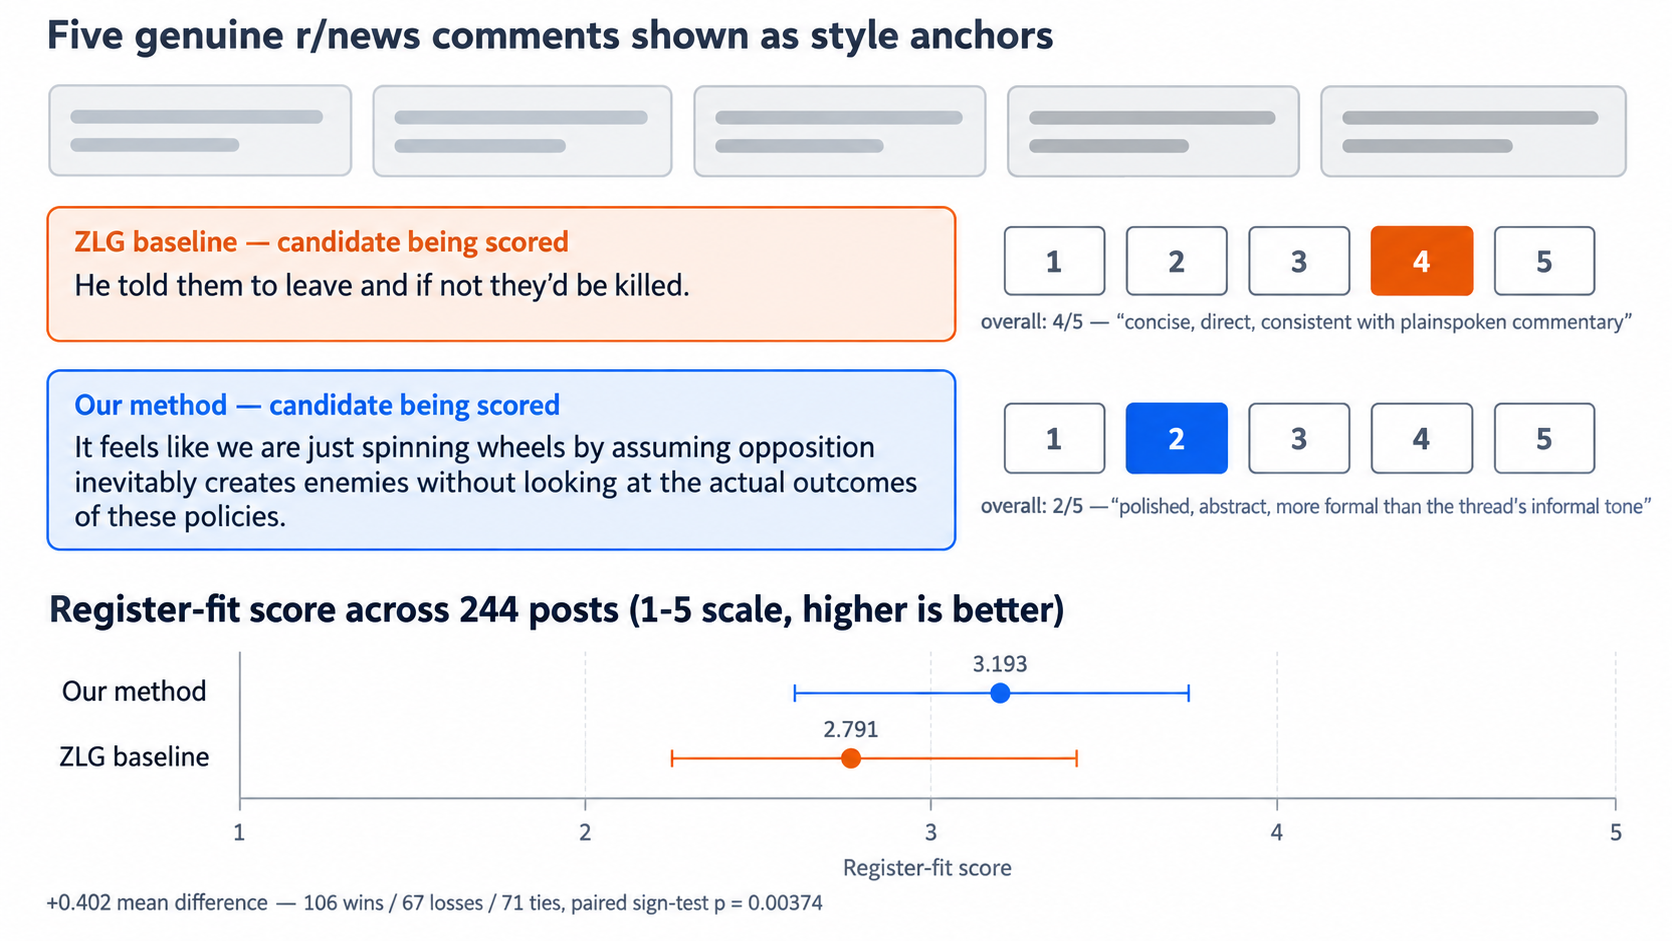
\includegraphics[width=\textwidth,height=0.55\textheight,keepaspectratio]{../common/figures/llm_judge_register_fit}
\caption{ملاءمة أسلوب التعليق للسياق. في المثال المعروض حصل \EN{ZLG}~\cite{lin2024zero} على \NUM{4/5} مقابل \NUM{2/5} لطريقتنا، بينما كان متوسط طريقتنا أعلى عبر \NUM{244} منشورًا (\NUM{3.193} مقابل \NUM{2.791}؛ اختبار إشارة مزدوج \NUMM{p=0.00374}).}
	\label{fig:judge-register}
\end{figure}
